%----------------------------------------------------------------------
%                        PROJECT DEFINITION
%----------------------------------------------------------------------
\renewcommand{\projnr}{A1}
\renewcommand{\projtitleshort}{Thermal annealing, evaporation, condensation}
\renewcommand{\projauth}{Lattard, Trieloff, Pucci}
%
\setcounter{section}{0}
\noindent{\normalfont\sffamily\Large\bfseries Project \projnr: \projtitleshort}
%
\section{Full title:}
\hspace{1\baselineskip}\\
\centerline{\large ``Laboratory experiments of thermal annealing,}\\
\centerline{\large evaporation and condensation of dust''}
%
\section{General information}\mbox{}

\subsection{Principle investigators:}
\hspace{-\baselineskip}\\\noindent
%
{\bfseries\itshape Lattard}, Dominique, Prof.~Dr.\\
C3, tenure\\
Date-of-birth: 4.4.1950, Nationality: French\\
DFG Code number of latest application: LA 1164/5-3\\
Mineralogisches Institut der Universit\"at Heidelberg\\
Im Neuenheimer Feld 236\\
69120 Heidelberg\\
Tel: 06221-544810\\
Fax: 06221-544805\\
Email: dlattard@min.uni-heidelberg.de\\
Private address:
Burgstr. 61, 69121 Heidelberg
Tel: 06221-473248\\
%
\vspace{1em}\\\noindent
{\bfseries\itshape Trieloff}, Mario, Priv. Doz. Dr. \\
non-tenure\\
Date-of-birth: 26.2.63, Nationality: German\\
DFG Code number of latest application: TR333/8-2\\
Mineralogisches Institut der Universit\"at Heidelberg\\
Im Neuenheimer Feld 236\\
69120 Heidelberg\\
Tel: 06221-546022\\
Fax: 06221-544805\\
Email: trieloff@min.uni-heidelberg.de\\
Private address:
Zaystr. 48, 76437 Rastatt
Tel: 07222/151875
%
\vspace{1em}\\\noindent
{\bfseries\itshape Pucci}, Annemarie, Prof. Dr.\\
C-3, tenure\\
Date-of-birth: 31.05.1954, Nationality: German\\
DFG Code number of latest application: PU 193/4-5\\
Kirchhoff-Institut f\"ur Physik\\
Im Neuenheimer Feld 227\\
69120 Heidelberg\\
Tel: 06221 549863\\
Fax: 06221 549869\\
Email: pucci@kip.uni-heidelberg.de\\
Private address: Gewann Husaren\"acker 47, 69121 Heidelberg, Germany\\
Tel: 06221 401089\\

\subsection{Co-investigators within this Forschergruppe:}
\begin{coilist}
\item H.~P.~Gail (ITA, Universit\"at Heidelberg)
\item W.~Tscharnuter (ITA, Universit\"at Heidelberg)
\item T.~Henning (MPIA, Heidelberg)
\end{coilist}


\section{Summary (Zusammenfassung)}
\subsubsection{Summary:} 
This project aims at obtaining reliable laboratory data on the
physico-chemical processes taking place during thermal annealing, evaporation
and condensation of silicate minerals. These data are urgently needed for a
consistent astrophysical modeling of radial abundances of dust/minerals and
the chemical composition of dust in protoplanetary disks. The dust component
determines the thermal structure of the disk, as radiative transfer depends
on optical properties of crystalline and amorphous minerals. Furthermore,
the chemical composition of solids and their abundance (Ca, Al rich
compounds, Mg-rich silicates, metal) determines the composition of accreting
solid bodies (terrestrial planets and asteroids). A variety of minerals -
particularly the cosmochemically abundant Mg-rich silicates of the olivine
and pyroxene groups - have been observed via infrared spectroscopy of
protoplanetary disks and comets. In this project, controlled evaporation and
condensation experiments (equilibrium, non-equilibrium) will be performed
under protoplanetary disk conditions and thermal annealing will be traced in
the laboratory by infrared spectroscopy of heated amorphous
materials. Experiments will focus on Mg-rich olivine and pyroxene with
variable Fe and Ca contents, and on Ca, Al compounds, for which reliable
data are still missing.

\subsubsection{Zusammenfassung:} 
Ziel des Projektes ist die experimentelle Ermittlung von Labordaten zu
physikalisch-chemischen Prozessen beim Ausheilen, Verdampfung und
Kondensation von Silikatmineralen. Diese Daten werden dringend ben\"otigt
f\"ur die konsistente Modellierung von radialen H\"aufigkeiten und die
chemische Zusammensetzung von Mineralstaub in protoplanetaren Scheiben. Die
Staubkomponente beeinflusst die thermische Strukur solcher Scheiben, da der
Strahlungstransport direkt an die optischen Eigenschaften von kristallinen
und amorphen Festk\"orpern gekoppelt ist.  Dar\"uberhinaus bestimmt die 
Zusammensetzung und H\"aufigkeit der verschiedenen Spezies (Ca,Al-Verbindungen, 
Mg-reiche Silikate, Metall) die Zusammensetzung der akkretierenden K\"orper
(z.B.\ Asteroide und terrestrische Planeten). Verschiedene Minerale -
haupts\"achlich die kosmochemisch h\"aufigen Mg-reichen Silikate der Olivin
und Pyroxen-Gruppe - sind mittels Infrarot-Spektroskopie in protoplanetaren
Scheiben und Kometen beobachtet worden. Innerhalb dieses Projektes sollen
kontrollierte Verdampfungs- und Kondensationsexperimente (Gleichgewicht,
Ungleichgewicht) unter Bedingungen durchgef\"uhrt werden, wie sie in
protoplanetaren Scheiben herrschen.  Thermisches Ausheilen wird im Labor
mittels Infrarot-Spektroskopie beim Aufheizen amorpher Materialien
gemessen. Die untersuchten Materialien werden sich konzentrieren auf solche
Mg-reichen Olivine und Pyroxene mit variablen Fe und Ca-Gehalten, sowie
Ca,Al Verbindungen, f\"ur die es bislang keine systematischen Untersuchungen
gibt.


\section{State of the art (Stand der Forschung)}

\subsection{Significance, processing and modelling of dust and minerals in protoplanetary disks}

Modeling of protoplanetary disks hitherto focussed on disk structure in
radial and - occasionally - vertical direction, and on temporal disk
evolution. Some models also consider gas phase chemistry in disks. On the
other hand, the physical state and chemical compositon of dust and the
variations in the abundances of specific minerals have not been studied
satisfactorily. Yet, the mineralogic-chemical composition of dust plays a
major role. The abundance of minerals and their spectroscopic properties
(mainly related to the degree of crystallinity) determine the opacity and
thermal structure of the disk, while the chemical composition of dust
determines the chemical compositions of solid bodies in the disk,
particularly of planetesimals, small asteroidal bodies and terrestrial
planets.

State of the art modelling of protoplanetary disks is summarized in
D'Alessio et al.\ (2005). Most models treat the dust properties
(e.g.\ opacity) rather schematically (Bell \& Lin, 1994; Bell et al.\ 1997),
while Gail (2001, 2004) and Wehrstedt \& Gail (2002, 2003) attempted to
achieve a self-consistent model of the dust component. Bergin et al.\ (2006)
review a number of theoretical studies of chemistry and mineralogy in
protoplanetary disks. Hydrodynamic 2-D and 3-D models of protoplanetary
disks which allow to study the importance of flows and mixing on the
chemistry in the disk are just becoming available (e.g.\ Klahr et al.\ 1999;
Turner et al.\ 2006).

All in all, today's computational capabilities allow more and more realistic
models of dust processing in protoplanetary disks. Such a development is
mandatory, the more as observations provide much more detailed constraints
on the minerals involved and/or their physical state, in particular their
crystallinity (see e.g.~review by Natta et al.~\cit{2006}). A variety of
minerals have been identified via infrared spectroscopy, and the study of
meteorites and interplanetary dust - including cometary dust (Wooden et al.\
2005, 2006) - offers detailed insights into the origin and processing of
solid matter in the early solar system. Basically, after cloud collapse,
interstellar dust enters the accretion disk. Studies of interstellar dust
(for a recent review see Tielens et al.\ 2005) indicate that amorphous
silicates are the main constituents, amorphous carbon is less abundant and
crystalline silicates are $<$2\% (Kemper et al.\ 2004, 2005).
%Such a small fraction contrasts model
%calculations that yield 5\% crystalline silicates in the ISM. 
%
%####{\bf [***** CHECK HERE *****]}
%
The low value may be partly caused by amorphization 
due to cosmic ray ion bombardment in the
interstellar medium. In the inner parts of a 
protoplanetary disk where temperatures
increase, amorphous dust anneals via intra-grain diffusion to form
crystalline dust, though shock annealing seems also a viable process
(cf.\ section below). In the inner part of the disk where the terrestrial
planets (and their precursor planetesimals) form, highly volatile species
(noble gases, CO, H$_{2}$O, CH$_{4}$, NH$_{3}$) are already gaseous, and
moderately volatile elements like Alkali, Zn etc. enter the gas phase via
evaporation. Successive devolatilization at higher temperatures in the inner
disk leaves more and more refractory residues (rich in refractory elements
such as Ca, Al). Temperature decrease (global or local, or related to
outward transport of matter) induces condensation of minerals, often
discussed in terms of classical condensation sequences: Refractory minerals
containing Ca, Al comprise oxides (corundum Al$_2$O$_3$, hibonite
Ca(Al,Ti,Mg)$_{12}$O$_{19}$, spinel MgAl$_2$O$_4$) and silicates (melilite -
solid solution of akermanite Ca$_2$MgSi$_2$O$_7$ and gehlenite
Ca$_2$Al$_2$SiO$_7$). They condense at higher temperatures than metal or the
Mg-silicates forsterite (Mg$_2$SiO$_4$) and enstatite (MgSiO$_3$) -- the
Mg-endmembers of the olivine and orthopyroxene solid solutions. At lower
temperatures, Ca, Al minerals can be converted into diopside
(CaMgSi$_2$O$_6$, a Ca-rich pyroxene) and anorthite (CaAl$_2$Si$_2$O$_8$,
the Ca-rich endmember of plagioclase feldspar solid solution), and Fe can
enter Mg-rich silicates. Volatile elements condense in the latest
compounds/minerals. Although Mg-rich silicates and metal contain the major
mass of condensible elements (in terrestrial planet forming regions), Ca, Al
silicates are major carriers for other important chemical elements that are
incompatible in olivine and orthopyroxene solid solutions. Moreover, Ca,Al
silicates and oxides are the main solids in regions where temperatures are
above the condensation temperatures of Mg-rich silicates. This makes their
study mandatory.

\subsection{Annealing of dust, crystalline silicates and radial mixing in protoplanetary discs}

Crystalline silicate dust has been observed in accretion disks of young
stellar objects (Meeus et al.\ 2001, Bouwman et al.\ 2001; van Boekel et
al.\ 2004; Molster et al.\ 2002; Apai et al.\ 2006). As dust in the
interstellar medium is mostly amorphous (Tielens et al.\ 2005), crystalline
dust has been interpreted as resulting from the crystallization of amorphous
dust at high temperatures during the preplanetary stage. This observation is
consistent with the identification of Mg-rich crystalline silicates
(forsterite, enstatite) in comets by infrared spectroscopy (Wooden et al.\
1999, 2000- Hale-Bopp; Deep impact: Harker et al.\ 2005), and with the
detection of isotopically solar-type silicates (forsterite) in anhydrous
interplanetary dust particles of presumably cometary origin (Messenger et
al.\ 2003). It is also consistent with the first results from the STARDUST
mission (cf.\ {\tt http://www.nasa.gov/stardust}). As cometary bodies formed
early and never experienced high temperatures (otherwise ultra-volatile
species like CO would have been lost) the presence of crystalline silicates
requires separate processing of this dust component before cometary
accretion. This might have taken place during the very early preplanetary
stage, most probably by annealing or condensation in the warmer inner
accretion disk and subsequent radial mixing into the outskirts or our solar
system where comets formed (see discussions by Wooden et al.\ 2005, 2006;
Alexander et al.\ 2006; Bergin et al.\ 2006). However, crystallization via
energetic processes like shock heating is also discussed (see Harker \&
Desch, 2002). Radial mixing of disk material is important for disk structure
and evolution (e.g.\ Morfill \& V\"olk, 1984). In recent years, more detailed
modelling of radial mixing processes were presented by Gail (2001, 2004),
Wehrstedt \& Gail (2002, 2003), Bockel\'ee-Morvan et al.\ (2002) and
Dullemond, Apai \& Walch~(\cit{2006}).

Detailed models of protoplanetary disks and the solar nebula should not only
consider accretion of amorphous dust, annealing, radial mixing processes and
the resulting radial distribution of crystalline material, but also the
implicit thermal disk structure governed by the extinction properties of the
dust component (Duschl et al.\ 1996; Gail, 1997; Gail, 2001, 2003; Wehrstedt
\& Gail, 2002, 2003; Bockel\'ee-Morvan et al.\ 2002), as extinction properties
are drastically reduced by annealing. This, however, needs more precise
kinetic studies and reliable parameters for thermal annealing retrieved from
laboratory experiments.

\subsection{Laboratory annealing studies}

The main process leading to the crystallization of amorphous cosmic dust is
thermal annealing. Previous laboratory studies have concentrated on the
thermally induced crystallization of amorphous pure Mg-silicates on the
composition of the Mg-olivine, forsterite (Mg$_{2}$SiO$_{4}$), or the
Mg-pyroxene, enstatite (MgSiO$_{3}$) (e.g.\ Hallenbeck et al.\ 1998; Brucato
et al.\ 1999; Fabian et al.\ 2000; Thompson et al.\ 2002; cf.\ also review in
Wooden et al.\ 2005). Up to now, there exist only very few exploratory
laboratory studies on the thermal annealing of Mg-Fe-silicates or of Ca-rich
pyroxenes and their results are only preliminary (e.g.\ Hallenbeck et
al.\ 1998; Brucato et al.\ 2002; Rotundi et al.\ 2002).

The progress of crystallization was usually monitored by mid-infrared
spectroscopy, in some studies conjointly with synchrotron X-ray diffraction
analysis (XRD) (e.g.\ Thompson et al.\ 2002 2003). Indeed, Infrared (IR)
spectroscopy is an important method in astro-mineralogical studies, not only
because it is most efficient to recognize silicate material in
protoplanetary disks. Optical phonons of minerals give rise to IR absorption
and emission spectra with lines that are characteristic for the chemical
composition, the atomic-geometrical structure, and the crystalline
symmetry. Furthermore, the line shape depends on the crystalline
quality. The size and shape of individual grains limits photon and phonon
waves and, therefore, leads to additional spectral changes. Numerous IR
measurements in the laboratory, performed by chemists, mineralogists, and
astrophysicists have yielded data on astrophysically relevant crystalline
substances, such as the mineral olivine - i.e.\ solid solution between the
forsterite and fayalite endmembers (e.g.\ Paques-Ledent \& Tarte, 1973;
Hofmeister, 1987, 1997; Reynard, 1991; J\"ager et al.\ 1998; Koike et al.\
2003) - the mineral group of the pyroxenes - in particular the solid
solution between the enstatite and ferrosilite endmembers, but also the
Ca-Mg pyroxene diopside (e.g.\ J\"ager et al.\ 1998; Koike et al.\ 2000;
Boffa Ballaran et al.\ 2001; Chihara et al.\ 2002) - , and few Ca, Al
minerals like spinel, diopside and melilite (Fabian et al.\ 2001; Koike et
al.\ 2000; Chihara et al.\ pers. comm.). IR data on diverse amorphous
substances (glasses, gels) on the composition of Mg-Fe-silicates are also
available (e.g.\ Stephens \& Russell, 1979; Dorschner et al.\ 1995; Scott \&
Duley, 1996; J\"ager et al.\ 1998, 2003).  In laboratory studies
characteristic annealing times were defined as the time necessary for the
first appearance of an ordered structure, $\tau_{S}$ (cf.\ Fabian et al.\
2000) or the one at which crystallization appears complete, $\tau_{C}$,
(cf.\ Brucato et al.\ 2002). Such characteristic annealing times ($\tau_{S}$
or $\tau_{C}$, in the following simply denoted as $\tau$ can be expressed
by the Arrhenius equation $\tau = \nu_{0}  \exp(-E_{a}/kT)$ (Fabian et al.\
2000), where $E_{a}$ is the effective activation energy, empirically
comprising nucleation and crystallization energy, and $\nu_{0}$ is a
constant proportional to the mean vibrational frequency of the silicate
lattice (Lenzuni et al.\ 1995). However, the literature results do not
display the expected linear trend in a $\ln \tau$ versus $1/T$ diagram, but
instead strongly scatter (Fig.\ 1). In case of the forsterite composition,
the three data points of Brucato et al.\ (2002) for complete crystallization
do point to a linear trend, but they do not match the results of Fabian et
al.\ (2000) (Fig.\ 1a). For the enstatite composition, only the data points
of Fabian et al.\ (2000) plot more or less on a line, whereas all other
results (from Hallenbeck et al.\ 1998; Brucato et al.\ 1999; Thompson et
al.\ 2002) do not show any temperature dependency and, in part, strongly
disagree (Fig.\ 1b). For instance, Nuth et al.\ (2000) claim, on the basis
of the data of Hallenbeck et al.\ (1998), that "crystalline olivine can be
produced from amorphous magnesium silicate at temperatures in the order of
1000 K within a month" whereas the results of Fabian et al.\ (2000) point to
complete crystallization at the same temperature within 12 hours.


\begin{figure}
\centerline{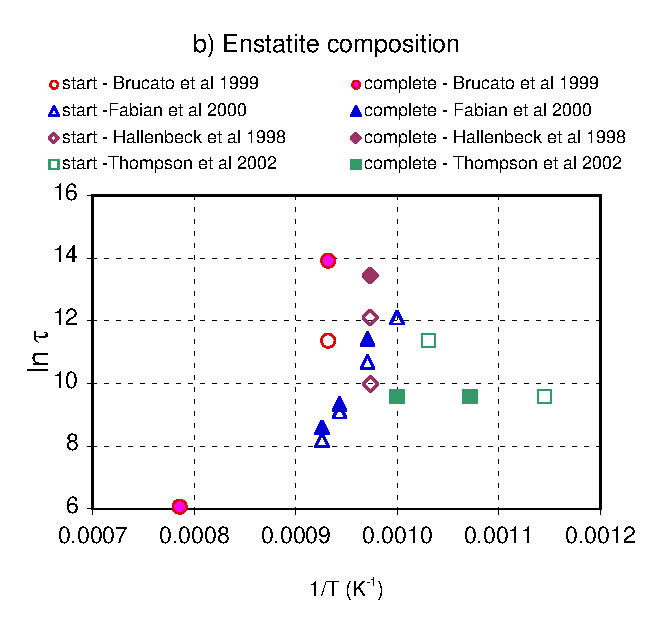
\includegraphics[width=8cm]{a1fig1a.eps}
\hspace{1em}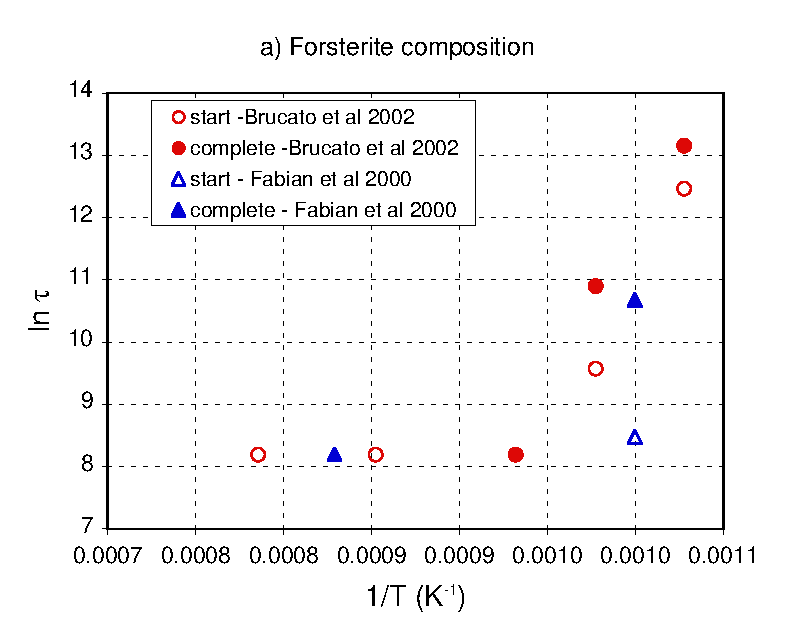
\includegraphics[width=8cm]{a1fig1b.eps}}
\caption{Characteristic annealing times ($\tau$) as a function of inverse
annealing temperature ($1/T$) for the bulk composition of forsterite (a) and
that of enstatite (b). Open symbols refer to annealing times necessary for
the first appearance of an ordered structure ($\tau_{S}$), filled symbols to
those at which crystallization appears complete ($\tau_{C}$). }
\end{figure}

\section{Preliminary work (Eigene Vorarbeiten)}

As an experimental mineralogist, PI Dominique Lattard has a longstanding
experience in high-temperature experiments in air, in vacuo or under
controlled oxygen fugacities (fO$_{2}$) on silicates and oxides, especially
on Fe-bearing phases. Such experiments were performed in the frame of very
different projects, e.g.\ to synthesize minerals, to simulate crystallization
processes from a silicate liquid, to determine the stability conditions of
single minerals or mineral assemblages as a function of temperature or
fO$_{2}$, to retrieve thermodynamic data or kinetic parameters (e.g.\ Langer
et al.\ 1977, Lattard \& Evans 1992, Lattard 1995, Lattard \& Partzsch 2001,
Lattard et al.\ 2005). D. Lattard has also the necessary expertise concerning
the mineralogical and chemical characterisation of products of
high-temperature experiments, i.e.\ with light microscopy, X-ray
diffractometry, scanning electron microscopy, electron microprobe analysis,
infrared spectroscopy, microscope-absorption-spectrophotometry, M\"ossbauer
spectroscopy (e.g.\ Langer et al.\ 1977, Langer \& Lattard, 1980, Lattard \&
Evans, 1992; Lattard 1995, Partzsch et al.\ 2004).

Co-PI Mario Trieloff has broad experience in cosmochemistry and
geochemistry, in particular with the isotope radiochronometry of processes
in the early solar system and their relationship to astrophysical processes
in protoplanetary disks. M. Trieloff conducted a number of studies on early
meteorite chronology and the accretionary history of planetesimals,
i.e.\ meteorite parent bodies (Trieloff et al.\ 2003; Pellas et al.\ 1997;
Korochantseva et al.\ 2005). He also studied processes that relate to disk
clearing and solar wind implantation into precursor planetesimals of
meteorite parent bodies and the terrestrial planets (Trieloff et al.\ 2000,
2002; Trieloff \& Kunz, 2005). Trieloff \& Palme (2006) reviewed and outlined
the early solar system history as seen by meteoriticists in the context of
astrophysical processes and disk evolution, written for and specifically
aimed at astrophysically oriented planetary scientists interested in
cosmochemistry. M. Trieloff has particular experience with high temperature
furnaces and ultra high vacuum technology for noble gas extraction from
solids, and mass spectrometric analysis, for which in-house constructed high
temperature furnaces are used. There is particular experience with general
diffusion theory (e.g.\ Trieloff et al.\ 2005), which is particularly
important if laboratory Arrhenius parameters (activation energy,
pre-exponential or frequency factor) are extrapolated from laboratory
temperature and times to parameters relevant in natural systems to be
modelled (where effects at much longer times and lower temperatures have to
be considered).

Co-PI Annemarie Pucci (before 1998 A. Lehmann) has a longstanding experience
with IR investigations of thin films with thickness in the nm range, both
with transmittance spectroscopy (for transparent substrates) and with IR
reflection of p-polarized light at grazing incidence (for metal
substrates). She used these techniques to gain information on morphology,
crystalline structure, chemical composition, impurities, and (in
semiconductors) free charge carriers of thin films (e.g.\ Lehmann et
al.\ 1982; Lehmann 1993; Priebe et al.\ 2004). In the last years A. Pucci and
her working group also studied the growth of metal films and of adsorbate
layers under UHV conditions. Important growth parameters were the metal
deposition rate adjusted via the temperature of a Knudsen cell and measured
with a quartz micro-balance and the substrate temperature. These two
parameters will be of importance in the evaporation/condensation
investigations planed in the present project. As a result of these previous
studies, the morphology development of metal growth on various substrates
was clarified and adsorbate structures could be explained (Lust et al.\ 2002;
Priebe et al.\ 2004; Pucci 2005). Also phase transitions in iron silicides
were monitored (e.g.\ Fahsold et al.\ 2002).

The amorphous thin films to be used in the annealing experiments will be
produced with the PLD setup at the Institut f\"ur Geologie, Mineralogie und
Geophysik, Ruhr-Universit\"at Bochum, in collaboration with Dr.\ Ralf Dohmen
and Prof.\ Dr.\ Sumit Chakraborty, who both have considerable experience with
thin films (both amorphous and crystalline thin films) of natural and
synthetic silicates, in particular of olivine and pyroxene compositions
(e.g.\ Dohmen et al.\ 2002).

For evaporation and condensation experiments, we envisage collaboration with
the leading expert Prof.\ H.\ Nagahara, University of Tokyo (Nagahara et
al.\ 1994; Nagahara and Ozawa 1996; Tsuchiyama et al.\ 1999; Tachibana et
al.\ 2002) and with Prof.\ S.\ Chakraborty and Dr.\ R.\ Dohmen, particularly
taking into account their previous studies (Dohmen et al.\ 1998, 2003; Dohmen
\& Chakraborty 2003) on the influence of crystal-parameters on reaction paths
and reaction rates, and considering diffusion effects.



%
% Here follows the own refereed publications by the PIs in relation to
% the project proposed here.
%
\ownpubltitle{Own publications related to the Forschergruppe:}
%
% BELOW IS ONLY AN EXAMPLE OF TWO ENTRIES. SEE THE ADDITIONAL FILES 
% SENT TO YOU WITH ALL THE REFERENCES FROM THE VORANTRAG
%
\begin{ownpubl}

\item Fahsold, G., Singer, K. and Pucci A. (2002) In-situ IR-transmission
  study of vibrational and electronic properties during the formation of
  thin-film $\beta$-FeSi$_2$. 
  \textit{Journal of Applied Physics\/}, \textbf{91}, 145
\item Korochantseva, E.V., Trieloff, M., Buikin, A.I., Meyer, H.P. and Hopp,
  J. (2005) Argon-40/Argon-39 dating, and cosmic ray exposure time of desert
  meteorites: Dhofar 300 and Dhofar 007 eucrites and anomalous achondrite NWA
  011. \textit{Meteoritics and Planetary Science\/}, \textbf{40}, 1433
\item Langer, K. and Lattard, D. (1980) Identification of a low-energy
  OH-valence vibration in zoisite. \textit{American Mineralogist\/},
  \textbf{65}, 779
\item Langer, K., Lattard, D. and Schreyer, W. (1977) Synthesis and
  stability of deerite, Fe$^{2+}$$_{12}$Fe$^{3+}$$_{6}$Si$_{12}$O$_{40}$ (OH)
  $_{10}$ and Fe$^{3+}$= Al$^{3+}$ substitutions at 15-28
  kb. \textit{Contributions to Mineralogy and Petrology \/}, \textbf{60}, 271
\item Lattard, D. (1995) Experimental evidence for the exsolution of
  ilmenite from titaniferous spinels. \textit{American Mineralogist \/},
  \textbf{80}, 968
\item Lattard, D. and Evans, B.W. (1992) New experiments on the stability of
  grunerite. \textit{European Journal of Mineralogy\/}, \textbf{4}, 218
\item Lattard, D. and Partzsch, G.M. (2001) Magmatic crystallization
  experiments at 1 bar in systems closed to oxygen: A new/old experimental
  approach. \textit{European Journal of Mineralogy \/}, \textbf{13}, 467
\item Lattard, D., Sauerzapf, U. and K\"asemann, M. (2005) New calibration
  data for the Fe-Ti oxide thermo-oxybarometers from experiments in the
  Fe-Ti-O system at 1 bar, 1000-1300 \degr C and a large range of oxygen
  fugacities. \textit{Contributions to Mineralogy and Petrology\/},
  \textbf{149}, 735
\item Lehmann, A. (1993) Information about the microcrystalline structure
  from the infrared reflection spectra of thin UV-optical films: NdF3 and
  MgF2. 
  \textit{Thin Solid Films\/}, \textbf{230}, 55
\item Lehmann, A., Schumann, L., Sobotta, H., Riede, V., Teschner, U. and
  H\"ubner, K. (1982) LO-TO Mode Splittings and Dynamic Effective Charges of
  Oxygen in Reactively Sputtered SiOx Determined by IR Spectroscopy. \textit{
  Physica status solidi (b) \/}, \textbf{111}, K103
\item Lust, A. Priebe, A., Fahsold, G. and Pucci, A. (2002) Infrared
  spectroscopic study of the CO-mediated decrease of the percolation threshold
  during the growth of ultrathin metal films on MgO(001). \textit{Surface and
  Interface Analysis \/}, \textbf{33}, 487
\item Partzsch, G.M., Lattard, D. and McCammon, C. (2004) M\"ossbauer
  spectroscopic determination of Fe$^{3+}$/Fe$^{2+}$ in synthetic basaltic
  glass: a test of empirical equations under superliquidus and subliquidus
  conditions. \textit{Contributions to Mineralogy and Petrology\/},
  \textbf{147}, 565
\item Pellas, P., Fieni, C., Trieloff, M. and Jessberger, E.K. (1997) The
  cooling history of the Acapulco meteorite as recorded by the 244Pu and
  40Ar-39Ar chronometers. \textit{Geochimica et Cosmochimica Acta\/},
  \textbf{61}, 3477
\item Priebe, A., Fahsold, G. and Pucci, A. (2004) Strong pyramidal growth
  of metal films studied with infrared spectroscopy. \textit{Journal of
  Physics and Chemistry\/}, \textbf{B 8}, 18178
\item Priebe, A., Walter, N. and Pucci, A. (2004) An IR spectroscopic study
  of silicon oxynitride films. In: \textit{Conference Digest of the 29th
  International Conference on Infrared and Millimeter Waves and of the 12th
  International Conference on Terahertz Electronics}, Karlsruhe, Germany,
  (Eds. M. Thumm, W. Wiesbeck), IEEE Catalog No.04X857, ISBN 0-78038490-3, 93
\item Pucci, A. (2005) IR spectroscopy of adsorbates on ultrathin metal
  films. \textit{Physica status solidi (b) \/}, \textbf{242}, 2704
\item Trieloff, M. and Kunz, J. (2005) Isotope systematics of noble gases in
  the Earth�s mantle: Possible sources of primordial isotopes and implications
  for mantle structure. \textit{Physics of the Earth and Planetary
  Interiors\/}, \textbf{148}, 13
\item Trieloff, M. and Palme, H. (2006) The origin of solids in the early
  solar system. In: \textit{Planet Formation - Theory, Observations, and
  Experiments}. (Eds. H. Klahr, W. Brandner), Cambridge University Press,
  Cambridge, 64
\item Trieloff, M., Falter, M., Buikin, A.I., Korochantseva, E.V.,
  Jessberger, E.K. and Altherr R. (2005) Argon isotope fractionation induced
  by stepwise heating. \textit{Geochimica et Cosmochimica Acta\/},
  \textbf{69}, 1253
\item Trieloff, M., Jessberger, E.K., Herrwerth, I., Hopp, J., Fi\'eni, C.,
  Gh\'elis, M., Bourot-Denise, M. and Pellas, P. (2003) 244Pu and 40Ar-39Ar
  thermochronometries reveal structure and thermal history of the H-chondrite
  parent asteroid. \textit{Nature\/}, \textbf{422}, 502
\item Trieloff, M., Kunz, J. and All\`egre, C.J. (2002) Noble gas systematics
  of the R\'eunion mantle plume source and the origin of primordial noble
  gases in Earth�s mantle. \textit{Earth and Planetary Science Letters\/},
  \textbf{200}, 297
\item Trieloff, M., Kunz, J., Clague, D.A., Harrison, D. and All�gre,
  C.J. (2000) The nature of pristine noble gases in mantle
  plumes. \textit{Science\/}, \textbf{288}, 1036

\end{ownpubl}
%
\section{Goals (Ziele)}
The main goal of the present project is to supply reliable laboratory data
on the physico-chemical processes taking place during evaporation,
condensation and thermal annealing of silicate minerals in proto-planetary
disks, with an emphasis on the kinetics of these processes. These data are
urgently needed for a consistent astrophysical modeling of the variations in
radial abundance of dust/minerals and of their chemical compositions at
various evolutionary stages of the protoplanetary disk. Studies will focus
on silicate minerals that are predicted by classical
condensation/evaporation sequences.  The project comprises two parts:

\begin{enumerate}
\item {\em Laboratory simulation of the crystallization} of amorphous silicate
components in cosmic dust during thermal annealing incl.\ determination of
reliable kinetic parameters. As the crystallization state of Fe-containing
olivine and pyroxene are expected to have the strongest influence on
extinction properties in protoplanetary disks, priority will be given to
forsterite-fayalite solid solution, and enstatite-ferrosilite solid
solution, but Ca-rich pyroxenes (diopside) will also be considered. Special
attention will be given to the preparation of amorphous material by
different methods (Pulsed Laser Deposition, glasses, gels).

\item {\em Laboratory determination of parameters for evaporation and
condensation} of dust/minerals under conditions relevant for protoplanetary
disks by heating and condensation experiments. Here, also some complementary
studies (where data are missing) will be performed on Fe-containing olivine
and pyroxene, but from the beginning we shall also focus on Ca, Al compounds
that are the only minerals in high temperature regions and important
carriers for many refractory elements at high temperatures (e.g.\ spinel,
hibonite, melilite, anorthite, diopside) and volatile elements at lower
temperatures (plagioclase, diopside). The first experiments will focus on
melilite solid solution of gehlenite-akermanite.

\end{enumerate}
%
These experiments are aimed to yield results for conditions relevant to
protoplanetary disks, e.g.\ temperature, redox state, pressure. An important
part to improve previous data are a) long-term experiments to get more
precise data for extrapolation to longer time intervals relevant in
protoplanetary discs b) extension of the experiments to cover more realistic
mineral compositions. Another improvement is attempted in the thorough
analytical characterization of starting materials and experimental outcome
material by micro-analytical tools like atomic force microscopy (AFM),
transmission and secondary electron microscopy (TEM; SEM), electron
microprobe (EMPA) and possibly ion microprobe (SIMS).

One of the strength of our project is the interdisciplinary cooperation
between astrophysicists, cosmochemists, mineralogists, experimental
physicists, who all contribute their specific expertise.


\section{Work schedule (Arbeitsprogramm)}
\subsection{Methods}
\subsubsection{Part 1 (Annealing):}

We plan to perform high-temperature (800-1200 K) annealing experiments on
iron-free and iron-bearing olivines - (Mg,Fe) $_{2}$SiO$_{4}$ -,
orthopyroxenes - (Mg,Fe)SiO$_{3}$ -, and clinopyroxenes - Ca
(Mg,Fe)Si$_{2}$O$_{6}$.

\paragraph{Amorphous starting materials:}

We shall particularly care for chemically homogeneous, structurally and
morphologically well-characterized amorphous starting materials. Our
emphasis will be on thin films produced by Pulsed Laser Deposition (PLD),
which fulfill these criteria in order to mimic amorphous cosmic dust. The
thin films will be produced with the PLD setup at the Institut f\"ur
Geologie, Mineralogie und Geophysik, Ruhr-Universit\"at Bochum, in
collaboration with Dr.\ Ralf Dohmen and Prof.\ Sumit Chakraborty.

The set up at Bochum has been custom designed for mineralogical applications
and includes an excimer Laser working with either ArF, KrF or XeF gas
mixtures, which leads to wavelengths of 193, 248 or 351 nm. For example,
with KrF the laser produces pulse energies up to 1400 mJ at a maximum
frequency of 50 Hz (pulse duration of 30 ns). The system can be operated at
high vacuum conditions of up to 10-5 Pa. This high vacuum background allows
the use of a flow of oxygen or of other gases with varying partial
pressure. This is of great advantage in order to avoid evaporation of Mg or
to control the redox condition of Fe (e.g.\ articles in Chrisey \& Hubler,
1994).

As targets for the laser beam, we shall essentially use dense pressed
polycrystalline pellets of the synthetic phase of interest, i.e.\ olivine,
pyroxene. In case of Fe$^{2+}$-bearing phases, these pellets will be
synthesized at high temperatures under oxygen fugacities controlled by
CO/CO$_2$ gas mixtures, in order to obtain the desired oxidation state of
iron (standard techniques in the working group of D. Lattard). We shall also
test high purity reagent mixtures (oxides, metals) on the desired
compositions.  As substrates to be coated with the thin films, we plan to
test spec. pure graphite, silicon crystal wafers, ceramic platelets
(e.g.\ Al$_{2}$O$_{3}$, ZrO$_{2}$) and synthetic polished and oriented single
crystals (commercially available, e.g.\ from Crystec GmbH).

Dohmen et al.\ (2002) have shown through thorough characterization with
different techniques (e.g.\ SEM, TEM, white light interference microscopy,
Rutherford Backscattering (RBS)) that the silicate thin films produced with
the PLD set up in Bochum are amorphous, highly uniform in thickness ($\pm$ 1
nm), chemically homogeneous and of the desired chemical composition. In some
cases the composition of the thin film is slightly more enriched in oxygen
than the target composition. Recent studies of the Bochum group have shown
that this problem may be corrected by reducing the background pressure in
the deposition chamber. This possibility is particularly important in case
of Fe-bearing compositions. In the mean time, amorphous thin films with
various Fe/Mg values on olivine and orthopyroxene compositions have been
routinely produced with the set-up in Bochum (Dohmen, pers. communication,
2006).

The first characterization of the amorphous thin films will be performed
with RBS, which enables measurements of both the chemical composition and
the thickness of the thin films (Dohmen et al.\ 2002). RBS measurements will
be carried out at the Dynamitron Tandem Laboratorium of the
Ruhr-Universit\"at Bochum in cooperation with Dr. Hans-Werner
Becker. Further characterization of the thin films with SEM and atomic force
microscopy (surface properties), with micro-analytical methods (chemistry)
and with IR spectroscopy will be performed at the mineralogical institute
and at the KIP.

For comparison we shall also use other homogeneous amorphous starting
materials, namely glasses and gels. Gels are relatively easily prepared
(e.g.\ Hamilton \& Henderson, 1968), but one has to take into account that
they contain iron in the trivalent state. In contrast, in Fe-bearing glasses
redox state of iron can be adjusted by equilibrating the silicate melt under
controlled fO$_{2}$ conditions in a furnace with a flowing CO/CO$_{2}$ gas
mixture (cf.\ Partzsch et al.\ 2004). Glasses in the Fe-Mg-Si-O system,
however, have to be prepared and examined with great care because of their
tendency to very rapidly crystallize during quenching (e.g.\ Boyd \& Schairer,
1964).

\paragraph{Annealing procedure}

We have two main options to realize annealing of the amorphous materials.
\begin{itemize}
\item Annealing at temperatures in the range 800-1200 K in vertical quench
furnaces under controlled atmosphere (air, CO/CO$_{2}$ gas mixtures) or in
vacuo (evacuated silica glass tubes) for well-defined run durations
(standard techniques at the Mineralogical Institute). Quench and subsequent
characterization of the run products with IR spectroscopy, X-ray
diffraction, and micro-analytical methods (SEM, electron microprobe, TEM,
etc.). Details on the experimental and analytical methods can be found
e.g.\ in Lattard et al.\ (2005).
\item Annealing in the experimental setup for IR spectroscopy under UHV
conditions (10$^{-8}$ Pa) at the KIP with in situ characterization of the
progress of crystallization of thin films with thickness in the nm range (up
to several 100 nm). Sample heating up to 1400 K is possible. Depending on
the sample size and the sample-holder construction, these temperatures can
be reached within seconds to minutes. Gas exposure (CO, CO$_{2}$, O$_{2}$)
up to a partial pressure of 2x10$^{-6}$ Pa can be performed in the UHV
chamber. The IR investigations of thin films can be performed either with
transmittance spectroscopy in the case of transparent substrates or with IR
reflection of p-polarized light at grazing incidence in the case of metal
substrates. Phonons in wafer-like samples with thickness in the micron range
and above are studied with reflectance spectroscopy. Above the phonon
absorption edge, transmittance studies can give information on impurities
and optical properties.
\end{itemize}

Even if annealing is performed in quench furnaces, IR investigations of thin
film run products can be performed in the experimental setup for IR
spectroscopy at KIP. In contrast to IR spectra retrieved from KBr pellets
(e.g.\ Brucato et al.\ 1999, Thompson et al.\ 2002), the artificial matrix
effects are avoided, giving clearer results on vibration properties. For
comparison, however, some IR spectra from powdered samples embedded in KBr
should also be measured in the sample chamber of the IR spectrometer at the
KIP and with other conventional IR spectrometers. We also plan in-situ
synchrotron IR investigations during annealing of short durations (e.g.\ at
temperatures around 1200 K) at the ANKA-Synchrotron (Karlsruhe).

To better define the progress of crystallization, we shall examine selected
annealed samples with the TEM, in collaboration with specialists
(Dr. F. Brenker, Universit\"at Frankfurt). We shall also analyze
recrystallized samples with RBS to exclude any reaction with the synthetic
substrates and to confirm that re-crystallization of the film is the only
process investigated.


\subsubsection{Part 2 (Evaporation/condensation):}

Experimental data for evaporation and condensation rates primarily exist
only for the Mg-rich silicates forsterite and enstatite. Few is known about
the important Fe-bearing olivine and pyroxene, or Ca, Al compounds, i.e.\ the
high temperature condensates corundum, hibonite, spinel, melilite, or at
slightly lower temperatures anorthite and diopside, and finally carrier
minerals of moderately volatile elements (e.g.\ Alkalis, Mn) like
plagioclase. For this reason, first experiments are planned on Fe-containing
olivine and pyroxene (Fo 60-100, En 60-100), and Ca, Al silicates (melilite
solid solution, diopside, plagioclase)

\begin{itemize}
\item As starting materials we will use either synthesized, commercially
available (e.g.\ Crystec GmbH, Berlin/ SPI supplies) or natural materials
(SPI Supplies/C.M. Taylor collection). They will be checked for homogeneity
and purity by EMP and possibly by ion microprobe. We expect to succeed in
obtaining appropriate material, however, in the case these materials have
not the desired level of homogeneity and purity, the synthesis of crystals
can also be performed by high temperature experiments under controlled
oxygen fugacity, either via solid state reactions or in the presence of a
melt phase or a flux. Respective high temperature furnaces are available at
the Mineralogical Institute, or via cooperations with labs specialized in
mineral synthesis.
\item Experiments with larger samples can be performed in ultra high vacuum
lines, using either resistance heated high temperature furnaces (up to 2000
\degr C) at the Min.\ Inst.\ or - alternatively - the experimental setup at
the KIP. This set up includes an electron impact heated furnace, from where
material can be evaporated and condensed as a thin film onto substrates that
are kept at specific temperatures. During condensation the film can be
characterized with IR spectroscopy. Gases (e.g.\ hydrogen) can be admixed on
both experimental facilities to simulate pressure and/or gas/dust ratios
relevant for protoplanetary disks. With this setup, partial pressures in the
UHV range, temperatures for evaporation up to 2000 K and for condensation up
to about 1400 K (see above) are possible. The photometric sensitivity is
sufficient to investigate phonon bands of condensed films with thickness in
the nm range. Evaporation rates are independently determined with a quartz
microbalance. The film morphology can be checked ex-situ with atomic force
microscopy (NanoScopeIV).
\item Equilibrium experiments with a Knudsen cell are necessary to clarify
phase relationships in some systems, e.g.\ for melilite solid solution with
the endmembers gehlenite and akermanite (evaporation dependent on chemical
composition and pressure, check for the occurrence of melts, check for
incongruent evaporation, see Hashimoto, 1990). Non-equilibrium experiments
(Langmuir configuration) to determine evaporation and condensation
coefficients will be performed afterwards. Evaporated material can be
condensed as thin films on a substrate kept at constant temperature. In the
case of olivine, phase relationships are principally clarified, however,
additional experiments at lower temperatures and longer laboratory times are
planned to verify and precise the kinetic parameters. Similarly, such
experiments must be performed for pyroxene solid solution between the
enstatite and ferrosilite endmembers. Particular attention has to be paid to
the control of oxygen fugacity. As an example oxygen fugacity can be
controlled by using a Mo capsule as Knudsen cell. Molybdenum reacts with
oxygen in the sample to form MoO$_{2}$. The fO$_{2}$ of the Mo-MoO$_{2}$
buffer is between that of the iron-w\"ustite (IW) and w\"ustite-magnetite
(WM) buffers (Mysen \& Kushiro 1988). The MoO$_{2}$ gas is not reactive
with the experimental system.
\item For the characterization of the experimental products a broad range of
micro-analytical facilities exists, e.g.\ atomic force microscopy at KIP or
optical and electron microscopy, electron microprobe, ion microprobe, X-ray
diffractometry at the Mineralogical Institute.
\end{itemize}
%
The experiments will be performed in collaboration with the leading expert
Prof. H. Nagahara, University of Tokyo. Cooperation is also envisaged with
Profs. S. Chakraborty and R. Dohmen, particularly taking into account their
previous studies (Dohmen et al.\ 1998, 2003; Dohmen \& Chakraborty 2003) that
have shown that crystal size or grain size of polycrystalline material
compared to the interacting reservoir also define reaction paths and, hence,
reaction rates. Moreover, diffusion may also play a role. Quantitative
modelling has to take into account these effects.



\subsection{Schedule Student 1 (Annealing)}
\subsubsection{First year}
Preparation and characterization (RBS, SEM, IR-spectroscopy) of amorphous
starting materials on the composition of Fe-free and Fe-bearing olivine,
(Fe,Mg) $_{2}$SiO$_{4}$, and of orthopyroxene, (Fe,Mg)SiO$_{3}$. The
emphasis will be on thin films prepared with the PLD method, but gels and
some Fe-bearing glasses should also be prepared for comparison.  First
annealing experiments in vertical quench furnaces. They will be performed in
air and in vacuum for Fe-free compositions, in vacuum and under different,
controlled oxygen fugacities for Fe-bearing compositions. Characterization
of the run products with RBS, SEM, EMP, IR-spectroscopy, TEM.  Preparation
and first tests of in-situ annealing in the experimental setup for IR
spectroscopy under UHV conditions and data analysis.

\subsubsection{Second year}
Preparation of amorphous starting materials on clinopyroxene compositions
(Ca(Fe,Mg) Si$_{2}$O$_{6}$). Further annealing experiments on different
compositions in quench furnaces and in the experimental setup for IR
spectroscopy under UHV conditions. Test of in-situ IR synchrotron
experiments at ANKA.


\subsubsection{Third year}
Final experiments. Extensive data analysis. Preparation of publications/PhD
thesis.

\subsection{Schedule Student 2 (Evaporation/Condensation)}
\subsubsection{First year}
Preparation and characterization of crystalline starting materials for
evaporation/ condensation experiments (Fe-containing olivine and pyroxene of
Fo 60-100, En 60-100, and Ca,Al silicates, i.e.\ melilite solid solution,
diopside, plagioclase). Evaporation/condensation experiments with Fe-bearing
olivine and pyroxene. Test of Ca, Al-bearing minerals and improvement of
experimental setup for high temperature experiments on Ca, Al minerals
(e.g.\ heating of condensation substrates). Characterization of condensation
products and evaporation residues by SEM, X-ray, electron microprobe, AFM,
and possibly also IRS. For this purpose, some experimental modification is
necessary regarding sample holder construction, and evaporator crucible
test.
\subsubsection{Second year}
Evaporation/condensation experiments for refractory Ca, Al bearing minerals.
\subsubsection{Third year}
Final experiments. Preparation of publications/PhD thesis.


\subsection{Literature}
%
% Here follows a general literature list related to the topic of the
% proposal, just like a literature list for a scientific paper.
%
% AGAIN ONLY EXAMPLES ARE LISTED NOW
%
\begin{literature}
\item Alexander, C.M.O., Boss, A.P., Keller, L.P., Nuth, J.A. and
  Weinberger, A. (2006) Astronomical and meteoritic evidence for the nature
  of interstellar dust and its processing in protoplanetary disks. In:
  \textit{Protostars and Planets V}, (Eds. B. Reipurth, D. Jewitt,
  K. Keil). \\ 
  {\tt http://ifa.hawaii.edu/UHNAI/ppv.htm}
\item All\`egre, C.J., Manh\`es, G. and Lewin, E. (2001) Chemical
  composition of the earth and the volatility control on planetary
  genetics. \textit{Earth and Planetary Science Letters\/}, \textbf{185}, 49
\item Apai, D. and Pascucci, I. and Bouwman, J. and Natta, A. and Henning,
  T. and Dullemond, C. P. (2005) The Onset of Planet Formation in Brown
  Dwarf Disks, \textit{Science\/}, \textbf{310}, 834
\item Bell, K.R., Cassen, P.M., Klahr, H.H. and Henning, T. (1997) The
  structure and appearance of protostellar accretion disks: limits on disk
  flaring. \textit{Astrophysical Journal\/}, \textbf{486}, 372
\item Bell, K.R. and Linn, D.N.C. (1994) Using FU Orionis outbursts to
  constrain self-regulated protostellar disk models. \textit{The Astrophysical
  Journal\/}, \textbf{427}, 987
\item Bergin, E.A., Aikawa, Y., Blake, D.A., and von Dishoeck, E.F. (2006)
  The chemical evolution of protoplanetary disks. In: \textit{Protostars and
  Planets V}, (Eds. B. Reipurth, D. Jewitt, K. Keil),\\ 
  {\tt http://ifa.hawaii.edu/UHNAI/ppv.htm}
\item Bockel\'ee-Morvan, D., Gautier, D., Hersant, F., Hur�, J.M., and Robert,
  F. (2002) Turbulent radial mixing in the solar nebula as the source of
  crystalline silicates in comets. \textit{Astronomy and Astrophysics\/},
  \textbf{384}, 1107
\item Boekel, R. van et al.\ (2004) The building blocks of planets within the
  'terrestrial' region of protoplanetary disks \textit{Nature\/},
  \textbf{432}, 479
\item Boffa Ballaran, T., Carpenter, M.A. and Ross, N.L. (2001) Infrared
  powder-absorption spectroscopy of Ca-free P21/c
  clinopyroxenes. \textit{Mineralogical Magazine\/}, \textbf{65}, 339
\item Boss, A. P. (2004) Evolution of the Solar Nebula. VI. Mixing and
  Transport of Isotopic Heterogeneity. \textit{Astrophysical Journal\/},
  \textbf{616}, 1265-1277
\item Bouwman, J., Meeus, G., de Koter, A., Hony, S., Dominik, C. and
  Waters, L.B.F.M. (2001) Processing of silicate dust grains in Herbig Ae/Be
  systems. \textit{Astronomy and Astrophysics\/}, \textbf{375}, 950-962.
\item Boyd, F.R. and Schairer, J.F. (1964): The system
  MgSiO$_{3}$-CaMgSi$_{2}$O$_{6}$. \textit{Journal of Petrology\/},
  \textbf{5}, 275
\item Bowen, N.L. and Schairer, J.F. (1935) The system
  MgO-FeO-SiO$_{2}$. \textit{American Journal of Science\/}, \textbf{29},
  151
\item Brucato, J.R., Colangeli, L., Mennella, V., Palumbo, P. and
  Bussoletti, E. (1999) Mid-infrared spectral evolution of thermally annealed
  amorphous pyroxene. \textit{Astronomy and Astrophysics\/}, \textbf{348},
  1012
\item Brucato, J.R., Mennella, V., Colangeli, L., Rotundi, A. and Palumbo,
  P. (2002) Production and processing of silicates in laboratory and in
  space. \textit{Planetary and Space Science\/}, \textbf{50}, 829
\item Chihara, H., Koike, C., Tsuchiyama, A., Tachibana, S., and Sakamoto,
  D. (2002) Compositional dependence of infrared absorption spectra of
  crystalline silicate. I. Mg-Fe pyroxenes. \textit{Astronomy and
  Astrophysics\/}, \textbf{391}, 267
\item Chrisey, D.B. and Hubler, G.K. (1994) Pulsed laser deposition of thin
  films, p. 613. John Wiley and Sons.
\item D'Alessio, P., Calvet, N. and Woolum, D.S. (2005) Thermal structure of
  protoplanetary disks. In: \textit{Chondrites and the protoplanetary disk\/},
  ASP Conf. Ser. Vol. 341 (Eds. A.N. Krot, E.R.D. Scott, B. Reipurth), 353
\item Dohmen, R. and Chakraborty, S. (2003) Mechanism and kinetics of
  element and isotopic exchange mediated by a fluid phase. \textit{American
  Mineralogist}, 88, 1251-1270.
\item Dohmen, R., Becker, H.-W., Meissner, E., Etzel, T. and Chakraborty,
  S. (2002) Production of silicate thin films using pulsed laser deposition
  (PLD) and applications to studies in mineral kinetics. \textit{European
  Journal of Mineralogy\/}, \textbf{14}, 1155
\item Dohmen, R. and Chakraborty, S. (2003) Mechanism and kinetics of
  element and isotopic exchange mediated by a fluid phase. \textit{American
  Mineralogist\/}, \textbf{88}, 1251
\item Dohmen, R., Chakraborty, S., Palme, H. and Rammensee, W. (1998)
  Solid-solid reactions mediated by a gas phase: An experimental study of
  reaction progress and the role of surfaces in the system olivine+iron
  metal. \textit{American Mineralogist\/}, \textbf{83}, 970
\item Dohmen, R., Chakraborty, S., Palme, H. and Rammensee, W. (2003) Role
  of element solubility on the kinetics of element partitioning: In situ
  observations and a thermodynamic kinetic model. \textit{Journal of
  Geophysical Research\/}, \textbf{108}, 2157
\item Dorschner, J., Begemann, B., Henning, T., J\"ager, C. and Mutschke,
  H. (1995) Steps toward interstellar silicate mineralogy. II.  Study of
  Mg-Fe-silicate glasses of variable composition. \textit{Astronomy and
  Astrophysics\/}, \textbf{300}, 503
\item {Dullemond}, C.~P., {Apai}, D. and {Walch}, S. (2006)
  Crystalline Silicates as a Probe of Disk Formation History, 
  \apjl \textbf{640}, 67
\item Duschl, W.J., Gail, H.P. and Tscharnuter, W.M. (1996) Destruction
  processes for dust in protoplanetary accretion disks. \textit{Astronomy and
  Astrophysics\/}, \textbf{312}, 624
\item Fabian, D., J\"ager, C., Henning, T., Dorschner, J. and Mutschke,
  H. (2000) Steps toward interstellar silicate mineralogy. V. Thermal
  evolution of amorphous magnesium silicates and silica. \textit{Astronomy and
  Astrophysics\/}, \textbf{364}, 282
\item Gail, H.P. (1997) Chemical reactions in protoplanetary disks IV. Multi
  component dust mixture. \textit{Astronomy and Astrophysics\/}, \textbf{332},
  1099
\item Gail, H.P. (2001) Radial mixing in protoplanetary accretion disks
  I. Stationary disk models with annealing and carbon
  combustion. \textit{Astronomy and Astrophysics\/}, \textbf{378}, 192
\item Gail, H.P. (2003) Formation and evolution of minerals in accretion
  disks and stellar outflows. In: \textit{Astromineralogy}, Lecture Notes in
  Physics (Ed. T. Henning) Springer, Heidelberg, 55
\item Gail, H.P. (2004) Radial mixing in protoplanetary accretion disks
  IV. Metamorphosis of the silicate dust complex. \textit{Astronomy and
  Astrophysics\/}, \textbf{413}, 571
\item J\"ager, C., Molster, F.J., Dorschner, J., Henning, T., Mutschke, H.,
  and Waters, L.B.F.M. (1998) Steps toward interstellar silicate
  mineralogy. IV. The crystalline revolution. \textit{Astronomy and
  Astrophysics\/}, \textbf{339}, 904
\item J\"ager, C., Dorschner, J., Mutschke, H., Posch, T., and Henning,
  T. (2003) Steps toward interstellar silicate mineralogy. VII.  Spectral
  properties and crystallization behaviour of magnesium silicates produced by
  the sol-gel method. \textit{Astronomy and Astrophysics\/}, \textbf{408}, 193
\item Hallenbeck, S. L.; Nuth, J. A. and Daukantas, P. L. (1998)
  Mid-Infrared spectral evolution of amorphous Magnesium silicate smokes
  annealed in vacuum: Comparison to cometary spectra. \ica, \textbf{131}, 198
\item Hamilton, D.L. and Henderson, C.M.B. (1968) The preparation of
  silicate compositions by a gelling method. \textit{Mineralogical
  Magazine\/}, \textbf{36}, 832
\item Harker, D.E. and Desch, S.J. (2002) Annealing of silicate dust by
  nebular shocks at 10 AU. \textit{Astrophysical Journal Letters\/},
  \textbf{565}, L109
\item Harker, D.E., Woodward, C.E., and Wooden, D.H. (2005) The dust grains
  from 9P/Tempel 1 before and after the encounter with deep
  impact. \textit{Science\/}, \textbf{310}, 278
\item Hashimoto, A. (1990) Evaporation kinetics of forsterite and
  implications for the early solar nebula. \textit{Nature\/}, \textbf{374}, 53
\item Hashimoto, A. (1991) Evaporation of melilite. \textit{Meteoritics\/},
  \textbf{26}, 344.
\item Hofmeister, A.M. (1987) Single-crystal absorptiobn and reflection
  infrared spectroscopy of forsterite and fayalite. \textit{Physics and
  Chemistry of Minerals\/}, \textbf{14}, 499
\item Hofmeister, A.M. (1997) Infrared reflectance spectra of fayalite, and
  absorption data from assorted olivines, including pressure and isotope
  effects. \textit{Physics and Chemistry of Minerals\/}, \textbf{24}, 535
\item J\"ager, C., Molster, F.J., Dorschner, J., Henning, T., Mutschke,
  H. and Waters, L.B.F.M. (1998) Steps toward interstellar silicate
  mineralogy. IV. The crystalline revolution. \textit{Astronomy and
  Astrophysics\/}, \textbf{339}, 904
\item J\"ager, C., Dorschner, J., Mutschke, H., Posch, T. and Henning,
  T. (2003) Steps toward interstellar silicate mineralogy. VII.  Spectral
  properties and crystallization behaviour of magnesium silicates produced by
  the sol-gel method. \textit{Astronomy and Astrophysics\/}, \textbf{408}, 193
\item Kemper F., Vriend W.J., Tielens A.G.G.M. (2004). The Absence of
  Crystalline Silicates in the Diffuse Interstellar
  Medium. \textit{Astrophys. J. \/}, \textbf{609}, 826
\item Kemper F., Vriend W.J., Tielens A.G.G.M. (2004). ERRATUM: The Absence of
  Crystalline Silicates in the Diffuse Interstellar
  Medium. \textit{Astrophys. J. \/}, \textbf{633}, 534
\item Klahr, H. H., Henning, Th. and Kley, W. (1999) On the Azimuthal
  Structure of Thermal Convection in Circumstellar
  Disks. \textit{Astrophysical J. \/}, \textbf{514}, 325-343.
\item Koch-Muller, M. (1997) Experimentally determined Fe-Mg exchange
  between synthetic staurolite and garnet in the system
  MgO-FeO-Al2O3-SiO2-H2O. \textit{Lithos\/}, \textbf{41}, 185
\item Koike, C., Tsuchiyama, A., Shibai, H., Suto, H., Tanab�, T., Chihara,
  H., Sogawa, H., Mouri, H. and Okada, K. (2000) Absorption spectra of Mg-rich
  Mg-Fe and Ca pyroxenes in the mid- and far-infrared
 regions. \textit{Astronomy and Astrophysics\/}, \textbf{363}, 1115
\item Koike, C., Chihara, H., Tsuchiyama, A., Suto, H., Sogawa, H. and
  Okuda, H. (2003) Compositional dependence of infrared absorption spectra of
  crystalline silicate. II. Natural and synthetic olivines. \textit{Astronomy
  and Astrophysics\/}, \textbf{399}, 1101
\item Lattard, D., Sauerzapf, U. and K\"asemann, M. (2005) New calibration
  data for the Fe-Ti oxide thermo-oxybarometers from experiments in the
  Fe-Ti-O system at 1 bar, 1000-1300�C and a large range of oxygen
  fugacities. \textit{Contributions to Mineralogy and Petrology\/},
  \textbf{149}, 735
\item Lindsley, D.H., Davis, B.T.C. and MacGregor, I.D. (1964) Ferrosilite
  (FeSiO3) synthesis at high pressures and temperatures. \textit{Science\/},
  \textbf{149}, 735
\item Meeus, G., Waters, L.B.F.M., Bouwman, J., van den Ancker, M. E.,
  Waelkens, C. \& Malfait, K. (2001) ISO spectroscopy of circumstellar dust in
  14 Herbig Ae/Be systems: Towards an understanding of dust processing,
  \textit{Astron. \& Astrophys. \/}, \textbf{365}, 476
\item Messenger, S., Keller, L.P., Stadermann, F.J., Walter, R.M., and
  Zinner, E. (2003) Samples of stars beyond the solar system: Silicate grains
  in interplanetary dust. \textit{Science\/}, \textbf{300}, 105
\item Molster, F.J., Waters, L.B.F.M., and Tielens, A.G.G.M. (2002)
  Crystalline silicate dust around envolved stars. II. The crystalline
  silicate complexes. \textit{Astronomy and Astrophysics\/}, \textbf{382}, 222
\item Morfill, G. E. and V\"olk, H. J. (1984) Transport of dust and vapor and
  chemical fractionation in the early protosolar cloud. \textit{Astrophysical
  J. \/}, \textbf{287}, 371-395
\item Mysen, B.O. and Kushiro, I. (1988) Condensation, evaporation, melting,
  and crystallization in the primitive solar nebula: Experimental data in
  the system MgO-SiO$_2$-H$_2$ to $1.0x10^{-9}$ bar and 1870\degr C with
  variable oxygen fugacity. \textit{American Mineralogist\/}, \textbf{73}, 1
\item Mysen, B.O. and Kushiro, I. (1989) Oxygen fugacity and evaporation
  phase relations in the solar nebula. \textit{Annual Reports of the
  Geophysical Laboratory\/}, 1988-1989, 33
\item Nagahara, H., Kushiro, I., and Mysen, B.O. (1994) Evaporation of
  olivine: Low pressure phase relations of the olivine system and its
  implication for the origin of chondritic components in the solar
  nebula. \textit{Geochimica et Cosmochimica Acta\/}, \textbf{58}, 1951
\item Nagahara, H. and Ozawa, K. (1996) Evaporation of forsterite in H2
  gas. \textit{Geochimica et Cosmochimica Acta\/}, \textbf{60}, 1445
\item Natta, A., Testi, L., Calvet, N., Henning, Th., Waters, L.\ B.\ F.\ M.
  and Wilner, D. (2006) Dust in Protoplanetary disks: properties
  and evolution. In: \textit{Protostars and Planets V}, (Eds. 
  B. Reipurth, D. Jewitt, K. Keil).\\ 
  {\tt http://ifa.hawaii.edu/UHNAI/ppv.htm} 
\item Nelson, R., Thiemens, M., Nuth, J. and Donn, B. (1989) Oxygen isotopic
  fractionation in the condensation of refractory smokes. \textit{Proceedings
  Lunar Planetary Sciene conference\/}, \textbf{19}, 559
\item Nuth, J.A., Rietmeijer, F.J.M., Hallenbeck, S.L., Withey, P.A. and
  Ferguson, F. (2000) Nucleation, growth, annealing and coagulation of
  refractory oxides and metals: Recent experimental progress and applications
  to astrophysical systems. In: \textit{Thermal emission spectroscopy and
  analysis of dust, disks, and regoliths}, ASP conference Series, Vol. 196,
  (Eds. M.L. Sitko, A.L. Sprague, D.K. Lynch), 313
\item Palme, H. (2001).Chemical and isotopic heterogeneity in protosolar
  matter. \textit{Phil. Trans. R. Soc. Lond.} \textbf{A 359}, 2061--2075.
\item Paques-Ledent, M.T. and Tarte, P. (1973) Vibrational studies of
  olivine type compounds. I. The IR and Raman spectra of the isotopic species
  of Mg2SiO4. \textit{Spectrochimica Acta\/}, \textbf{29A}, 1007
\item Partzsch, G.M., Lattard, D. and McCammon, C. (2004) M\"ossbauer
  spectroscopic determination of Fe3+/Fe2+ in synthetic basaltic glass: a test
  of empirical fO2 equations under superliquidus and subliquidus
  conditions. \textit{Contributions to Mineralogy and Petrology\/},
  \textbf{147}, 565
\item Reynard, B. (1991) Single-crystal infrared reflectivity of pure
  Mg$_2$SiO$_4$ forsterite and (Mg0.86,Fe0.14)2SiO$_4$ olivine - new data and a
  reappraisal. Physics and Chemistry of Minerals\/, \textbf{18}, 19
\item Rotundi, A., Brucato, J.R., Colangeli, L., Ferrini, G., Mennella, V.,
  Palomba, E. and Palumbo, P. (2002) Production, processing and
  characterization techniques fo cosmic dust analogues. \textit{Meteoritics
  and Planetary Science\/}, \textbf{37}, 1623
\item Scott, A. and Duley, W.W. (1996) Ultraviolet and Infrared refractive
  indices of amorphous silicates. \textit{The Astrophysical Journal\/},
  \textbf{105}, 401
\item Smith, D. (1971) Stability of the assemblage iron-rich
  orthopyroxene-olivine-quartz. \textit{American Journal of Science\/},
  \textbf{271}, 370
\item Stephens, J.R. and Russel, R.W. (1979) Emission and extinction of
  ground and vapor-condensed silicates from 4 to 14 microns and the 10 micron
  silicate feature. \textit{The Astrophysical Journal\/}, \textbf{228}, 780
\item Tachibana, S., Tsuchiyama, A., and Nagahara, H. (2002) Experimental
  study of incongruent evaporation kinetics of enstatite in vacuum and in
  hydrogen gas. \textit{Geochimica et Cosmochimica Acta\/}, \textbf{66}, 713
\item Thompson, S.P., Fonti, S., Verrienti, C., Blanco, A., Orono, V., and
  Tang, C.C. (2002) Laboratory study of annealed amorphous MgSiO3 silicate
  using IR spectroscopy and synchrotron X-ray diffraction. \textit{Astronomy
  and Astrophysics\/}, \textbf{395}, 705
\item Thompson, S.P., Fonti, S., Verrienti, C., Blanco, A., Orono, V., and
  Tang, C.C. (2003) Crystalline comet dust: Laboratory experiments on a simple
  silicate system. \textit{Meteoritics and Planetary Science\/}, \textbf{38},
  457
\item Tielens A.G.G.M., Waters L.B.F.M. and Bernatowicz T.J. (2006) Origin
  and evolution of dust in circumstellar and interstellar environments. In:
  \textit{Chondrites and the protoplanetary disk\/}, ASP Conf. Ser. Vol. 341
  (Eds. A.N. Krot, E.R.D. Scott, B. Reipurth), 605.
\item Trieloff, M. and Palme, H. (2006) The origin of solids in the early
  solar system. In: \textit{Planet Formation - Theory, Observations, and
  Experiments}, (Eds. H. Klahr, W. Brandner), Cambridge University Press,
  Cambridge, 64
\item Tsuchiyama, A., Tachibana, S. and Takahashi, T. (1999) Evaporation of
  forsterite in the primordial solar nebula; rates and accompanied isotopic
  fractionation. \textit{Geochimica et Cosmochimica Acta\/}, \textbf{63}, 2451
\item Turner, N. J., Willacy, K., Bryden, G. and Yorke, H. W. (2006)
  Turbulent Mixing in the Outer Solar Nebula. \textit{Astrophysical J. \/},
  \textbf{ 639}, 1218-1226.
\item Wang, J., Davis, A.M., Clayton, R.N. and Hashimoto, A. (1999)
  Evaporation of single crystal forsterite: Evaporation kinetics, magnesium
  isotope fractionation, and implications of mass-dependent isotopic
  fractionation of a diffusion-controlled reservoir. \textit{Geochimica et
  Cosmochimica Acta\/}, \textbf{63}, 953
\item Wehrstedt, M. and Gail, H.P. (2002) Radial mixing in protoplanetary
  accretion disks. II. Time dependent disk models with annealing and carbon
  combustion. \textit{Astronomy and Astrophysics\/}, \textbf{385}, 181
\item Wehrstedt, M. and Gail, H.P. (2003) Radial mixing in protoplanetary
  accretion disks V. Models with different element mixtures. \textit{Astronomy
  and Astrophysics\/}, \textbf{410}, 917
\item Wooden, D.H., Harker, D., Woodward, C.E., Butner, H.M., Koike, C.,
  Witteborn, F.C. and McMurtry, C.W. (1999) Silicate mineralogy of the dust in
  the inner coma of comet C/1995 01 (Hale-Bopp) pre- and
  post-perihelion. \textit{The Astrophysical Journal\/}, \textbf{517}, 1034
\item Wooden, D.H., Butner, H.M., Harker, D.E. and Woodward, C.E. (2000)
  Mg-rich silicate crystals in comet Hale-Bopp: ISM relics or solar nebula
  condensates? \textit{Icarus\/}, \textbf{143}, 126
\item Wooden, D.H., Harker, D.E. and Brearley, A.J. (2005) Thermal
  processing and radial mixing of dust: Evidence from comets and primitive
  chondrites. In: \textit{Chondrites and the protoplanetary disk}, ASP
  Conference Series, Vol. 341 (Ed. A.N. Krot, E.R.D. Scott, B. Reipurth), 774
\item Wooden, D. H., Desch, S., Harker, D., Gail, H.-P. and Keller,
  L. (2006) Comet grains and Implications for Heating and Radial Mixing in the
  Protoplanetary Disk. In: \textit{Protostars and Planets V}, (Eds. 
  B. Reipurth, D. Jewitt, K. Keil).\\ 
  {\tt http://ifa.hawaii.edu/UHNAI/ppv.htm}
\end{literature}



\section{External/International collaborations}
\begin{collablist}
\item[Bochum] Prof. Dr. Sumit Chakraborty and Dr. Ralf Dohmen (Institut f\"ur
Geologie, Geophysik und Mineralogie, Ruhr-Universit\"at Bochum) have
considerable experience with the production and characterization of
amorphous thin silicate films (in particular on olivine and pyroxene
compositions) and crystallization rates of amorphous films. They have
contributed fundamental studies to silicate reaction kinetics (e.g.\ applying
Knudsen cell experiments) and are leading experts in the field of
diffusion-controlled processes in silicates.
\item[Frankfurt] PD Dr. Frank Brenker is leader of the "Nanogeoscience" group at the
Intitut f\"ur Geowissenschaften of the Universit\"at Frankfurt. He is an
expert in the use of transmission electron microscopy (TEM) to reconstruct
the thermo-mechanical history of crystals in terrestrial and
extraterrestrial materials. He is also involved in the chemical
characterization of presolar dust particles in the frame of the STARDUST
mission.
\item[Tokyo] Prof. Dr. H. Nagahara, University of Tokyo: Dr. Nagahara is a
leading expert in experimental simulation of evaporation and condensation
processes related to the early solar system.
\item[Jena] Dr. C. J\"ager, Dr. H. Mutschke, University of Jena: Leading
experts on IR spectroscopy of astrophysically relevant minerals.
\end{collablist}



\section{Link to other projects of the Forschergruppe}
\begin{linkproj}
\item[A2] There will be strong immediate interaction with project A2
(W.M. Tscharnuter/H.-P. Gail/ T. Henning), as the data on mineral processing
will be used to model the evolution of dust/minerals in protoplanetary
discs, and implicitly the radial distribution of chemical elements that will
determine the composition of accreting planetesimals and planets. In turn
the model calculations of project A2 will provide the information which
minerals are present in the disk and therefore should be investigated.
\item[D1] The chronometry of chondrule and planetesimal formation (project
D1 - M. Trieloff, R. Altherr, T. Stephan) places constraints on the time
scales to establish differences in chemical compositions
(refractory/volatile and forsterite/enstatite and metal/silicate
fractionation) of the solids due to evaporation/condensation processes. Such
fractionations are only effective during small grain processing. At a later
stage of evolution, once mm to cm-sized objects have formed and been
incorporated into larger planetesimals, no more significant modifications
are expected via solid-gas reactions. Another important part is linked to
the STARDUST results, which will yield data on the abundance of refractory
and/or crystalline solids in comets. The physical conditions associated with
the origin of these components is evaluated in A1 and will - implicitly -
constrain the extent of radial mixing into comet forming regions in the
outer solar system.
\item[D2] 
% Another direct link is given to the project D2 by
% S. Wolf/C.P. Dullemond, as distributions of different mineral dust species
% can be calculated on the base of experimental data. Predicted distributions
% of mineral species, their state (crystalline/amorphous) and composition, can
% be used to evaluate observational parameters (e.g.\ appropriate IR spectra -
% spatially resolved with corresponding mineral features) that serve to trace
% the evolutionary state of protoplanetary disks.
Dust opacity measurements made in A1 can be used in D2. A1 also provides
annealing, evaporation and condensation data that allow A2 to calculate
mineral distributions for D2.
\item[B3] Coagulation experiments with mixtures of different mineral species
in B3 (J.\ Blum / M.\ Trieloff) will be prepared according to the radial
abundances predicted by A2 using the A1 results. The preparation of mineral
grain separates strongly uses know how, equipment and materials that are
synthesized and/or prepared in this project (A1).
\item[B1/B2] The long term perspective of these projects is also to envisage
coagulation experiments with multi-mineral mixtures, relying on A1 expertise
\end{linkproj}



\section{Team members (Zusammensetzung der Arbeitsgruppe)}
%
% NOTE: Only list non-DFG-funded team members.
% NOTE: Also list technical assistents, students etc involved in the project
%
\subsection*{Mineralogical Institute}
\begin{teamlist}
\item[Prof. Dr. Dominique Lattard , principle investigator]\mbox{}\\
Team leader of the experimental mineralogy group: Supervision of PhD student
1, assistant supervision of PhD student 2.
\item[Priv. Doz. Dr. Mario Trieloff,  principle investigator]\mbox{}\\
Team leader of noble gas isotope geochronology group. Supervision of PhD
student 2, assistant supervision of PhD student 1, transfer of results into
project A2, establishing the link to early solar system processes derived
from cosmochemistry (e.g.\ basic cosmochemical fractionation processes).
\item[Dr. Michael Burchard]\mbox{}\\ 
Scientist in the high-pressure high-temperature laboratory: Assistance
during high-temperature synthesis or annealing experiments.
\item[Dr. W. Schwarz, Dr. J. Hopp]\mbox{}\\
Noble gas mass spectrometry laboratory, Mineralogical Institute: Assistance
in high temperature vacuum furnace experiments, and ultra high vacuum
technology
\item[Dr. H.-P. Meyer]\mbox{}\\
Electron microprobe laboratory, Mineralogical Institute: Assistance in SEM
work and electron microprobe analysis
\item[Dipl. Phys. Th. Ludwig]\mbox{}\\ 
Secondary Ion microprobe laboratory, Mineralogical Institute: Assistance in
ion microprobe analysis
\item[3 technicians (Mechanic, Electrician, Polishing Lab)]
\end{teamlist}

\subsection*{Kirchhoff Institute for Physics}
\begin{teamlist}
\item[Prof. Dr. Annemarie Pucci, principle investigator]\mbox{}\\
Team leader of the Surface Science Group at the KIP: Co-supervision of PhD
students 1 and 2.
\item[Dipl. Phys. Robert Lovrincic (doctorate student until December 07)]
\item[Dipl. Phys. Frank Neubrech (doctorate student until April 08)]\mbox{}\\ 
These doctorate students are involved in other projects, but they can give
assistance to the PhDs of this project in their work at KIP.
\item[Post doc, N.N., from 2007 (successor Dr. G. Fahsold)]\mbox{}\\
The Surface Science Group gets support from the KIP workshops and management
team.
\end{teamlist}

\subsection*{Institut f\"ur Theoretische Astrophysik}
\begin{teamlist}
\item[Tscharnuter, W. M., Prof. Dr. (ITA, C4): co-investigator]\mbox{}\\
Numerical hydrodynamics, radiative transfer, modeling of accretion disks,
modeling of chemistry.
\item[Gail, H.-P., Prof. Dr. (ITA, Wiss. Ang): co-investigator]\mbox{}\\
Modeling of mineralogical processes and of gas phase chemistry, modeling of
accretion disks and radiative transfer
\end{teamlist}


\subsection*{Max-Planck-Institut f\"ur Astronomie (Heidelberg)}
\begin{teamlist}
\item[Henning, Prof. Dr. (MPIA, C4): co-investigator]\mbox{}\\
Modeling of dust extinction, chemistry in accretion disks,
analysis of observations of accretion disks and 
mineralogy of dust.
\end{teamlist}


\vspace{1em}

\section{Funding requested}
We request funding for two PhD student positions for this project. 
The following table gives the full overview of 
requested funding:\vspace{1\baselineskip}\\
%
% The table that follows is the overview over the full requested 
% funding, including the positions, travel, consumables and ``other
% costs'' (which might include transportation costs of radioactive
% material or the rent of a drop tower or such).
%
\centerline{\begin{tabular}{||l|l|l|l||} \hline \hline & Year 1 & Year 2 &
Year 3 \\ 
\hline 
Personnel: 2 PhD-students (E13/2) & 48.000 & 48.000 & 48.000 \\
Personnel: 3 student research assistants & 8500 & 8500 & \\
(20 hours/month each) &  &  &  \\
Consumables & 16.250 & 16.250 & 10.000 \\
Travel &   4.046 &   4.046 &   1.368 \\
Investments & 27.000 & - & - \\
Other costs &  9.250 &   9.250 &   7.250 \\
\hline
{\bf Total:} & 103.046 & 86.046 & 66.618  \\
\hline
\hline
\end{tabular}
}
\mbox{}\vspace{1em}\\
Below these costs are explained in more detail:

\subsection{Personnel (Personalbedarf)}
The present project cannot be realized without the working power of two
qualified young scientists who will perform quite different, complementary
tasks:
\begin{teamlist}
\item[PhD-Student 1 (annealing) (E13/2)]\mbox{}\\
%
This student will prepare the amorphous starting materials for the annealing
experiments, i.e.\ gels and glasses, as well as the crystalline olivine and
pyroxene samples used as targets for the PLD method. He/she will perform the
annealing experiments and characterize both the starting materials and the
annealing products with various methods (XRD, IR, RBS, SEM, EMP,
TEM). Together with the supervisors he/she will analyze the data and
interpret the results.  The ideal candidate for this position should be
highly motivated, have a solid background in mineralogy, preferably with
some experience in experimental mineralogy and analytical work (e.g.\ in the
frame of her/his master or diploma work) and be willing to learn a lot about
thin films and different spectroscopic methods.
%
\item[PhD-Student 2 (evaporation and condensation) (E13/2)]\mbox{}\\
%
This student will have the task to select appropriate materials (natural
and/or synthetic materials, some of them possibly in-house synthesized) check
of chemical homogeneity (SEM, ion microprobe), preparing the final
experimental setup (heating/condensation), conducting
evaporation/condensation experiments. The initial stages require close
cooperation with Prof. H. Nagahara at Tokyo university.
\end{teamlist}
Both PhD students will be very busy with learning the fundamentals and
practical aspects of the methods to be used in the present project and with
gaining the scientific background for interpretation of the required data
set. Each of them will need the help of a student research assistant to
perform routine work: e.g.\ preparation of starting materials for the
synthesis of glasses or crystalline materials, documentation of the samples
prior to microprobe work, recalculation of microprobe analysis. Another
student assistant experienced in experimental physics is needed to assist
setup of the experimental facilities at the KIP, and subsequent routine work
to maintain the experiments.  Therefore we ask for 3 student assistants each
for 20 hours per month for the first 2 years.

\subsection{Consumables (Verbrauchsmaterial)}
\begin{enumerate}
\item \textbf{Experiments at KIP (Group of A. Pucci)}\\
\begin{expenseslistnarrow}
Crucibles, AFM tips, IR windows, IR polarizer, filaments, chemicals, sample
holder material, ultra-pure gases, sapphire plates, ceramics, UHV feed
troughs       & \EUR   & \hfill 8 000 \\
\textbf{Total} & \EURBF & \hfill \textbf{8 000} 
\end{expenseslistnarrow}
%
\item \textbf{Experiments in the high-temperature vacuum extraction line
(Noble gas lab at Mineralogical Institute (Group M. Trieloff)}\\
\begin{expenseslistnarrow}
Tantalum crucibles and thermocouples for resistance 
heated furnace & \EUR & \hfill   2 500\\
Glass furnaces (kovar or duran), incl. W/Re thermocouple 
and Mo crucible & \EUR &  \hfill 2 200\\
Glass ware, chemical agents for sample purification
(ethanole, quarzdistilled water, nitric acid) & \EUR  & \hfill 400\\
Working gases (oxygen, argon, methane) & \EUR &  \hfill  800\\
Consumable materials  (mass spectrometer filament, 
pump maintenance) &\EUR & \hfill 200\\
Thermocouples to monitor getter heating & \EUR & \hfill 300\\
Copper / gold wires & \EUR & \hfill 800\\
\textbf{Total} & \EURBF &   \hfill \textbf{7 200}
\end{expenseslistnarrow}

\item \textbf{Experiments in the high-temperature laboratory at the
  Mineralogical Institute (Group D. Lattard)}\\
\begin{expenseslistnarrow}
Chemicals for syntheses & \EUR &\hfill  300\\
High purity gases for the control of the oxygen fugacity 
(CO2: 250 �/bottle; CO 750 �/bottle) & \EUR & \hfill 2 500\\
EMF sensor, ceramic tubing, heating elements & \EUR & \hfill 3 000 \\
Pt-Pt90Rh10 thermocouple wire & \EUR & \hfill 500\\
Sample holders and capsules: Pt wire, Pt foil, 
  AgPd and Au tubing etc. & \EUR & \hfill 4 000 \\
\textbf{Total} & \EURBF & \hfill  \textbf{10 300}
\end{expenseslistnarrow}

\item \textbf{Consumables for SEM and EMP (Mineralogical Institute)}\\
\begin{expenseslistnarrow}
Filaments, pumping oil, graphite for coating, gas, paper for videoprinter, 
spectrometer windows & \EUR & \hfill 4 500\\
Preparation of polished sections: diamond paste, saw blade
 $ \EUR $ \hfill  500\\
\textbf{Total} & \EURBF & \hfill \textbf{5 000}
\end{expenseslistnarrow}

\item \textbf{Other consumables}\\
\begin{expenseslistnarrow}
Synthetic polished and oriented single crystal 
substrates for thin films from Crystec GmbH, SPI Supplies.
10 x 10 mm ca 15-30 Eur/piece &  \EUR & \hfill   2 000\\
\textbf{Total} & \EURBF & \hfill\textbf{2 000}
\end{expenseslistnarrow}

\begin{expenseslistnarrow}
\hline
\textbf{Consumables 1st + 2nd year are equally distributed, in 3rd year lower because experimental work mostly completed:}
\textbf{Total consumables 1st + 2nd year:} & \EURBF  &  \hfill \textbf{32 500}\\
\textbf{Consumables (Verbrauchsmaterial) (3rd year)}
  & \EURBF & \hfill \textbf{10 000}\\
\hline
\end{expenseslistnarrow}

\end{enumerate}


\subsection{Travel expenses in addition to Project Z (Reisekosten)}
%
% Here only travel expenses not related to usual regular Forschergruppe
% meetings and the overall per capita budget for conferences.
%
\begin{expenseslist}
PhD student 1 will have to spend  3 times 1 week in Bochum (S. Chakraborty,
R. Dohmen) in the first two years to prepare part of the starting materials
and to perform Rutherford backscattering measurements. 
(21 days $\times$ (24\EUR/day+50\EUR/night)+3$\times$160 \EUR train)
& \EUR & \hfill 2 034\\
%
PhD student 1 will have to spend about 6 weeks in Frankfurt (F. Brenker) in
the first two years for TEM analysis of annealed materials.
(42 days $\times$ (24\EUR/day+50\EUR/night)+6$\times$40\EUR train)
& \EUR &\hfill 3 348\\
%
PhD student 2 will visit Tokyo University (H. Nagahara) to check experimental 
setup of evaporation experiments, and conduct test runs in preparation for the 
Heidelberg setup
10 days $\times$ (41\EUR/day+113\EUR/night)+1$\times$1200\EUR flight)
& \EUR &\hfill 2 710 \\
%
\textbf{Total in first 2 years} & \EURBF & \hfill \textbf{8 092}\\
%
PhD student 1 will spend about 3x 4 days in Jena (H. Mutschke, C. J\"ager) 
to exchange and  discuss results. 
(12 days $\times$ (24\EUR/day+50\EUR/night)+3$\times$160\EUR train)
& \EUR & \hfill 1 368\\
%
\textbf{Total in last year} & \EURBF &\hfill \textbf{1 368}
\end{expenseslist}



% Estimated cost per year:\vspace{1\baselineskip}\\
% \centerline{\begin{tabular}{|p{18em}|p{7em}|p{7em}|}
% \hline
% ?   &  \hfil ?              & \hfil ? \\
% \hline
% ?   &  \hfil ?              & \hfil ? \\
% \hline
% \end{tabular}}

\subsection{Investments}
\begin{expenseslist}
(KIP, A. Pucci) MCT-IR broadband detector with improved longterm stability -
is required for mid-IR spectra acquisition during slow thin-film
formation/evaporation over more than 2 h, obtained material data needed for
astrophysical modelling & \EUR &\hfill 9 000\\
%
(KIP, A. Pucci) Two appropriate power supplies (for sample heating and for
evaporation) - presently used power supplies are insufficient to achieve
high temperatures necessary for Ca, Al minerals & \EUR & \hfill 9 000\\
%
(MIN, M. Trieloff) Vacuum pump for UHV furnace - this UHV furnace capable to
reach temperatures of about 2300 K was built in anticipation of this
project, estimated costs EUR 15 000 (construction materials only, without
personnel costs) - the vacuum pump could not yet be afforded 
& \EUR & \hfill 9 000\\
%
\textbf{Total} & \EURBF & \hfill \textbf{27 000}
\end{expenseslist}

\subsection{Other costs (Sonstige Kosten)}
\subsubsection{Other costs for the first 2 years}\mbox{}\\
Other costs 1st + 2nd year are equally distributed \\
\begin{expenseslist}
MIN PhD student 1: Use of the PLD set up in Bochum: 500 \EUR/day
 & \EUR & \hfill 3 000 \\
%
MIN PhD student 1:RBS measurements at the Dynamitron Tandem
Laboratorium of the Ruhr-Universit\"at Bochum: 500 \EUR/day
 & \EUR & \hfill 4 000 \\
%
MIN PhD student 1: TEM investigations: 250 \EUR/day 
 & \EUR & \hfill 2 500 \\
%
MIN PhD student 1: Preparation of thin foils with the Focussed Ion
Beam technique for TEM investigations (commercial) 
 & \EUR & \hfill 8 000 \\
%
KIP (A. Pucci): Access to databases and software for analysis 
 & \EUR & \hfill 1 000 \\
%
\textbf{Total} & \EURBF & \hfill \textbf{18 500}
\end{expenseslist}

\subsubsection{Other costs for the 3rd year}\mbox{}\\
\begin{expenseslist}
TEM investigations: & \EUR & \hfill  1 250 \\
%
Preparation of thin foils with the Focussed Ion Beam technique for TEM
investigations (commercial) & \EUR & \hfill 5 000 \\
%
KIP (A. Pucci): Access to databases and software for analysis 
 & \EUR & \hfill 1 000 \\
%
\textbf{Total} & \EURBF & \hfill \textbf{7 250}
\end{expenseslist}


% Estimated cost per year:\vspace{1\baselineskip}\\
% \centerline{\begin{tabular}{|p{15em}|p{10em}|p{7em}|} 
% \hline
% ?  & \hfil ? & \hfil ? \\
% \hline
% \end{tabular}}




\section{Preconditions for carrying out the project at home institution}
%
% This is one of the main subsections of a DFG Normalverfaren proposal.
% Several of the subsubsections in this subsection we have placed in their
% own subsections above (like team members, collaborations). What remains
% are the following three subsections. For those not familiar with these,
% we refer to the DFG Merkblatt on Normalverfahren-proposals.
%
\subsection{Scientific equipment available (Apparative Ausstattung)}
%
% Please list those larger instrument available to you for the project (if
% applicable also larger computer equipment in case you need substantial
% amounts of computer time).
%
\subsubsection{KIP, A.Pucci's group:}
For the project one of the two FTIR spectrometers coupled to an UHV chamber
will be used. The UHV chambers are equipped with an electron diffraction set
up (LEED, or RHEED), with a quartz microbalance for calibration of the
deposited mass, with evaporators (physical evaporation from a small Knudsen
cell), mass spectrometer and spectroscopy option in the visible
range. Within the project also the NanoScopeIV atomic force microscope will
be available.

\subsubsection{Mineralogical Institute:}
\begin{compactitemize}
\item Noble gas laboratory: Various ultra high vacuum furnace types: induction heated glass furnaces, resistance heated double vacuum furnaces with Ta-crucibles for sample heating 
\item SEM (Leo 440)  with energy dispersive system 
\item Electron microprobe CAMECA SX51
\item Laboratory for mineral separation (milling, magnetic and heavy  liquid separation), optical microscopes, binocular
\item Experienced mechanical and electronics workshop  
\item Ion microprobe CAMECA 3 mf for trace element analysis, lateral resolution 10-30(m 
\item High-temperature, high-pressure laboratory
\item 3 vertical quench furnaces (up to 1300 resp. 1500�C)
\item Box furnace (up to 1500�C)
\item Gas mixing device with electronic valves
\item Xray-diffractometers (Phillips, Siemens D500) 
\end{compactitemize}


\subsection{Institution's general contribution (Laufende Mittel f\"ur Sachausgaben)}
%
% Please state the annual fund for consumables which comes from the
% institution's budget or any other third party  (please list separately) to
% pay for the research for which your project is part of.  Use estimates where
% applicable. 
%
We estimate that the running costs per year of our equipment
are:\vspace{1\baselineskip}\\
%
\centerline{\begin{tabular}{|p{18em}|p{7em}|}
\hline
Kirchhoff Institut f\"ur Physik:       & \hfill 3 000 \\
\hline
Mineralogical Institute:               & \hfill 2 000\\
\hline
\end{tabular}}\vspace{1em}\\
which will be contributed by the institutes



